\documentclass{article} % decribes the type of document
\usepackage{graphicx} % images
\graphicspath{ {./../pix/} } % set the default location of images
\usepackage{geometry} % change default margins
\usepackage{underscore} % underscores
\usepackage{multicol} % side by side list and figures
\usepackage{ulem} % shorthand for \uline (underline)
\usepackage{listings} % add code to document
\usepackage[hidelinks]{hyperref} % for hyperlinks
\usepackage[utf8]{inputenc} % no idea
\usepackage[english]{babel} % no idea
\usepackage[]{amsthm} % no idea
\usepackage[]{amssymb} % no idea
\usepackage{xcolor} % for colors
\definecolor{Maroon}{RGB}{178, 0, 0}
\definecolor{DarkGreen}{RGB}{3, 168, 97}
\usepackage{xurl} % fixes hbox error for long urls
\usepackage{caption} % for bold and italic figure captions
\usepackage{nomencl} % for nomenclature page
\usepackage{amsmath} % for equation blocks w/o numbers
\usepackage{tabularx} % for tables
\usepackage{adjustbox} % for smaller tables

% Fancy Math for rounding symbols
\usepackage{mathtools, nccmath}
\DeclarePairedDelimiter{\nint}\lfloor\rceil

\DeclarePairedDelimiter{\abs}\lvert\rvert

% Listings styles packages defined in ./listingsstyles.tex
\usepackage{listingsstyles}
\makenomenclature % for nomencl page
\bibliographystyle{ieeetr} % for bibliography in the IEEE format

% Define nomenclature groups
\usepackage{etoolbox}
\renewcommand{\nomgroup}[1]{%
    \item[\bfseries
    \ifstrequal{#1}{S}{Symbols}{%
    \ifstrequal{#1}{A}{Acronyms}{}}%
]}
\geometry{
    left=1.0in,
    right=1.0in,
    top=1.0in,
    bottom=1.0in,
    a4paper,
%    showframe % Show the layout of the page
}
% Comment out sections that you don't want to compile
\includeonly{
    chapters/bounty,
    chapters/week20,
    chapters/week19,
    chapters/week18,
    chapters/week17,
    chapters/week16,
    chapters/week15,
    chapters/week14,
    chapters/week13,
    chapters/week12,
    chapters/week11,
    chapters/week10,
    chapters/week9,
    chapters/week8,
    chapters/week7,
    chapters/week5,
    chapters/week4,
    chapters/week3,
    chapters/week2,
    chapters/week1,
    chapters/references
}


\title{\vspace{5cm}The Network Times}
\author{Ian Turner}

\begin{document}
\lstset{language=[LaTeX]TeX} % Set the language as TeX or LaTeX for listings

\maketitle

%\newpage
%\tableofcontents
%
%\newpage
%\addcontentsline{toc}{section}{Nomenclature}
%\label{sec:nomenclature}
%\printnomenclature
%
%\newpage
%\addcontentsline{toc}{section}{List of Figures}
%\listoffigures
%
%\newpage
%\addcontentsline{toc}{section}{List of Tables}
%\listoftables

\newpage
%%%%%%%%%%%%%%%%%%%%%%%%%%%%%%%%%%%%%%%%%%%%%%%%%%%%%%%%%%%%%%%%%%%%%%%%%%%%%%%
\section{Bounty Submission for Balajis on Farcaster}
%%%%%%%%%%%%%%%%%%%%%%%%%%%%%%%%%%%%%%%%%%%%%%%%%%%%%%%%%%%%%%%%%%%%%%%%%%%%%%%

Balaji put out a
\textcolor{purple}{\href{https://warpcast.com/balajis.eth/0x218b92a7}{cast}} on
Wednesday the 6th challenging anyone to create an AI NYT. He provided a nice
example of something working
\textcolor{blue}{\href{https://twitter.com/balajis/status/1601398685106991105?s=46}{18
months ago}} with inferior LLM models. I've been looking for a reason to stay up
all night coding, so I figured I'd give it a shot.


\subsection*{Why \LaTeX\ Ian?}
Great question anon! I write these notes everyday at work and on other projects
since pmarca gave me the idea with his ANTI-TODO list concept. Blog is no longer
on the internet or else I would link it here. This may be completely useless to
people, but I don't really but much detail in my git commits (I should start) so
maybe this will help if you end up contributing.

\newpage
%%%%%%%%%%%%%%%%%%%%%%%%%%%%%%%%%%%%%%%%%%%%%%%%%%%%%%%%%%%%%%%%%%%%%%%%%%%%%%%
\section{Week 20}
%%%%%%%%%%%%%%%%%%%%%%%%%%%%%%%%%%%%%%%%%%%%%%%%%%%%%%%%%%%%%%%%%%%%%%%%%%%%%%%

\subsection*{Sunday, 10/13/2024}
\begin{itemize}
    \item i fell off !!!!
    \item that's okay, been busy with work
    \item added filter to bb, still haven't deployed yet rofl
\end{itemize}

\newpage
%%%%%%%%%%%%%%%%%%%%%%%%%%%%%%%%%%%%%%%%%%%%%%%%%%%%%%%%%%%%%%%%%%%%%%%%%%%%%%%
\section{Week 19}
%%%%%%%%%%%%%%%%%%%%%%%%%%%%%%%%%%%%%%%%%%%%%%%%%%%%%%%%%%%%%%%%%%%%%%%%%%%%%%%

\subsection*{Saturday, 9/05/2024}
\begin{itemize}
    \item this has just evolved into my personal project notes for me to yap to
        myself.
    \item i still really like thenetworktimes idea, but am too lazy to seperate
        smaller project notes into other documents.
    \item i'll just roll with this and work on the bryptoblogs site since it's
        been down for a month or so at this point (rip)
\end{itemize}

\subsection*{Sunday, 9/06/2024}
\begin{itemize}
    \item i need to work on bryptoblogs, scripts still work somehow, still
        haven't set up a con job to automate this stuff oopsie.
\end{itemize}

\newpage
%%%%%%%%%%%%%%%%%%%%%%%%%%%%%%%%%%%%%%%%%%%%%%%%%%%%%%%%%%%%%%%%%%%%%%%%%%%%%%%
\section{Week 18}
%%%%%%%%%%%%%%%%%%%%%%%%%%%%%%%%%%%%%%%%%%%%%%%%%%%%%%%%%%%%%%%%%%%%%%%%%%%%%%%

\subsection*{Monday, 9/09/2024}
\begin{itemize}
    \item shit i need to grind harder what am i doing.
    \item anyways, let's try to deploy leptos brypto blogs now, server is just
        down hahaha have not pointed domain back to old vercel one.
    \item okay, fr, fundementally i never understood what \texttt{cargo leptos
        watch} (from the  
        \textcolor{blue}{\href{https://github.com/leptos-rs/cargo-leptos}{cargo leptos}}
        build tool) was doing.
    \item i would do a few release build just to test the compile times, but i
        never did anything more.
    \item looking at the fly io deployment example from the book, i simply
        forgot to incorporate the tailwind build step and thought it would just
        magically work somehow. luckily i can just run the help command or read
        the examples.
    \item wow... i've many skill issues related to nginx!!!
    \item much to think about.
\end{itemize}

\subsection*{Tuesday, 9/10/2024}
\begin{itemize}
    \item hard stuck on deploying leptos 0.6 app and migrating to 0.7, so i'll
        just work on features that should work either way.
    \item should brain dump some github issues soon... there is much to do (not 
        in a rush obvi or i wouldn't be using leptos at all)
    \item ...
\end{itemize}

\newpage
%%%%%%%%%%%%%%%%%%%%%%%%%%%%%%%%%%%%%%%%%%%%%%%%%%%%%%%%%%%%%%%%%%%%%%%%%%%%%%%
\section{Week 17}
%%%%%%%%%%%%%%%%%%%%%%%%%%%%%%%%%%%%%%%%%%%%%%%%%%%%%%%%%%%%%%%%%%%%%%%%%%%%%%%

\subsection*{Monday, 8/26/2024}
\begin{itemize}
    \item added simple grep over the users desired channels (hardcoded for now).
    \item i really need to stop putting of the shuttle thing and just implement
        it. it's probably really hard and this is going to stink but whatever,
        i'm sure i'll learn a ton.
    \item ...
\end{itemize}

\newpage
%%%%%%%%%%%%%%%%%%%%%%%%%%%%%%%%%%%%%%%%%%%%%%%%%%%%%%%%%%%%%%%%%%%%%%%%%%%%%%%
\section{Week 16}
%%%%%%%%%%%%%%%%%%%%%%%%%%%%%%%%%%%%%%%%%%%%%%%%%%%%%%%%%%%%%%%%%%%%%%%%%%%%%%%

\subsection*{Saturday, 8/17/2024}
\begin{itemize}
    \item trying to add redis cache for user data in cast entry; getting molly
        wopped (?) by the borrow checker currently.
    \item okay it's compiling now, but i'm using it improperly.
    \item okay it's working as designed now lets gooo!
    \item i am going to leave the remote feature branches up since i reference
        them in issues, and will help contributors if that ever is a thing.
\end{itemize}

\subsection*{Sunday, 8/18/2024}
\begin{itemize}
    \item that was really easy to get working, but it literally conflicts with
        my lazy loading logic which was based on the user scrolling (before
        caching was implemented) so this clearly breaks things.
    \item i'll need to try to get some sort of client side cache working as
        well, it might be a RIP to the wasm bundle size but oh well, perhaps the
        bundle splitting lads will fix by the time i have a usable app.
    \item omg that was also very easy, now first load on any feed is unusable!!!
        but every subsequent load is lightning which is exactly what i expected
        to happen.
    \item luckily my website is a nice LLM enjoyer, crypto adjacent power app
        that has a questionable use case! :)
    \item again, all these hacks are fun to implement, but really, i should be
        migrating to leptos 0.7 beta since it allows axum to actually do work in
        paralled (i think), in 0.6, even the server functions somehow only run
        blocking on 1 thread if i am not mistaken.
    \item much to do, after 0.7 migration, think about postgres rust shuttle
        like service implementation (rip).
\end{itemize}


\newpage
%%%%%%%%%%%%%%%%%%%%%%%%%%%%%%%%%%%%%%%%%%%%%%%%%%%%%%%%%%%%%%%%%%%%%%%%%%%%%%%
\section{Week 15}
%%%%%%%%%%%%%%%%%%%%%%%%%%%%%%%%%%%%%%%%%%%%%%%%%%%%%%%%%%%%%%%%%%%%%%%%%%%%%%%

\subsection*{Monday, 8/05/2024}
\begin{itemize}
    \item added bio to profile component, now need to add the casts by fid
        endpoint, i don't even think the current site has this, but i built it
        months ago on the old hubble server so i'll just use it now.
    \item i tried to add the casts by fid endpoint in another server function on
        the profile page but failed miserably and was just left with a hanging
        request and i am not good enough with leptos to understand why hahaha. i
        suspect i am doing too much in a single component and i should just
        create a new one similar to the home page, render the cast list but pass
        in the cast from the user rather than the channel for each cast in the
        list.
    \item ...
\end{itemize}

\subsection*{Friday, 8/09/2024}
\begin{itemize}
    \item added writers room idea i've been thinking about for a while, much to
        do, and change to merge the old blocking article gen with this new
        streaming idea which allows for fast iteration on an idea for an
        article, or meme, or whatever really.
    \item ...
\end{itemize}

\newpage
%%%%%%%%%%%%%%%%%%%%%%%%%%%%%%%%%%%%%%%%%%%%%%%%%%%%%%%%%%%%%%%%%%%%%%%%%%%%%%%
\section{Week 14}
%%%%%%%%%%%%%%%%%%%%%%%%%%%%%%%%%%%%%%%%%%%%%%%%%%%%%%%%%%%%%%%%%%%%%%%%%%%%%%%

\subsection*{Thursday, 8/01/2024}
\begin{itemize}
    \item damn i need to commit more here!
    \item working on cast list and cast entry merging finally. implemented very
        lazy lazy loading. i still don't have shuttle postgres thing set up so i
        have to make all these fetches randomly, so i'd like to keep them to a
        minimum for user data.
    \item this lazy load feature was fun since it gave me an excuse to use some
        \texttt{web_sys} stuff related to interactive observers.
    \item i basically have it so that only the first 8 cast entries load data
        immediately (user data, not cast body), and the rest are loaded as they
        become visible in the viewport.
    \item this was a breeze with this fine grained readtivity business honestly!
    \item the IntersectionObserver types are cracked since i can set a threshold
        for visibility (i used 10 percent in this feature). 
\end{itemize}

\subsection*{Saturday, 8/03/2024}
\begin{itemize}
    \item working on
        \textcolor{blue}{\href{https://github.com/iturner72/thenetworktimes/issues/3}{issue
        3}} and realized that \texttt{create_server_action} seemed interesting
        but not needed since it works well with an ActionForm and i don't really
        need one at the moment. it's nice to know that it's easy enough to add
        though later for like a tweetdeck style fetch.
    \item added images, will wait on reactions until i can get cast creation 
        working i think.
\end{itemize}

\subsection*{Sunday, 8/04/2024}
\begin{itemize}
    \item working on the pfp page and will continue to issue max  
        \textcolor{blue}{\href{https://github.com/iturner72/thenetworktimes/issues/4}{issue 4}}
    \item will study leptos routes since rn things are just really shitty and
        not organized.
    \item oh it's just \texttt{:id} for the path in the route i can use for
        profile, very nice.
    \item i decided to use \texttt{create_memo} for the fid on the profile page
        which uses a params map as a prop, this allows flexibility later i
        think...
    \item either way, i needed to handle the \texttt{ServerFnError} manually in
        the create resourse call for \texttt{user_data}, i should probably use
        the leptos helper libs in the ecosystem, but i feel like doing all these
        annoying manual things helps me learn what the framework is actually
        doing, so i don't mind the extra dev time.
    \item ...
\end{itemize}

\newpage
%%%%%%%%%%%%%%%%%%%%%%%%%%%%%%%%%%%%%%%%%%%%%%%%%%%%%%%%%%%%%%%%%%%%%%%%%%%%%%%
\section{Week 13}
%%%%%%%%%%%%%%%%%%%%%%%%%%%%%%%%%%%%%%%%%%%%%%%%%%%%%%%%%%%%%%%%%%%%%%%%%%%%%%%

\subsection*{Sunday, 7/21/2024}
\begin{itemize}
    \item working on the cast list and profile components after dealing with
        alchemy annoyances and switched to infura for eth l1 and optimism l2.
    \item still need to deploy the leptos app soon, but i at least want to
        replicate what's already live.
    \item ...
\end{itemize}

\subsection*{Wednesday, 7/24/2024}
\begin{itemize}
    \item going to clean up the profile component today and think about how to
        make the fetches and plan for just db queries.
\end{itemize}

\newpage
%%%%%%%%%%%%%%%%%%%%%%%%%%%%%%%%%%%%%%%%%%%%%%%%%%%%%%%%%%%%%%%%%%%%%%%%%%%%%%%
\section{Week 12}
%%%%%%%%%%%%%%%%%%%%%%%%%%%%%%%%%%%%%%%%%%%%%%%%%%%%%%%%%%%%%%%%%%%%%%%%%%%%%%%

\subsection*{Thursday, 7/11/2024}
\begin{itemize}
    \item working on a home page in the leptos rewrite which compines the
        channel and cast list components together side by side. this is so janky
        on moblie, but having fun with leptos fine grained stuff on the hovers
        on desktop web.
\end{itemize}

\newpage
%%%%%%%%%%%%%%%%%%%%%%%%%%%%%%%%%%%%%%%%%%%%%%%%%%%%%%%%%%%%%%%%%%%%%%%%%%%%%%%
\section{Week 11?}
%%%%%%%%%%%%%%%%%%%%%%%%%%%%%%%%%%%%%%%%%%%%%%%%%%%%%%%%%%%%%%%%%%%%%%%%%%%%%%%

\subsection*{Thursday, 7/04/2024}
\begin{verbatim}
{} 
|| 
||   .,,;;;;;;,,.. 
||.;;;;;;*;;;;;;;*;;, ..,,;;;;;;%%%%%, 
||';*;;;;;;;;*;;;;;;,::*::;;;*;;%%%%%%>>%%%%%,                 .; 
|| ';;;;;*;;;;;;;;*;;,:::::*;;;;;@@@##>>%%%%%%,        ..,,;%%%%' 
||  ;*;;;;;;;;*;;;;;;,::*;:;;;;*;@@@@##ooO0@@##>>%%%%%%%%%%%%%%' 
||  ;;;;;;*;;;;;;;;*;;,:;:::*;;;;%%%%%%ooO0@@##>>%%%%%%%%%%a@@' 
||  ;;*;;;;;;;;;*;;;;;,::*;::;;;*;%%%%%%>>%%%%%%ooO@@@@@@@@@@@ 
||  ;;;;;;*;;;;;;;;*;;,:::::;*;;;;@@@@##>>%%%%%%%ooO@@@@@@@@%% 
||  ;;*;;;;;;;;;*;;;;;;,::*;:;;;*;@@@@@##ooO0@@##>>%%%%%%%%%%% 
||  ;;;;;;;*;;;;;;;*;;;,:::::*;;;;;%%%%%%ooO0@@@##>>%%%%%%%%a@, 
||  ;;;*;;;;;;;;*;;;;;;,::*:;;;;;*;%%%%%%%>>%%%%%%%%ooO@@@@@@@@ 
||  ;;;;;;;*;;;;;;;;*;;;,::::;*;;;;@@@@@##>>%%%%%%%%%ooO@@@@@%%' 
||  ;;*;;;;;;;;*;;;;;;;;,::*:;;;:;*;@@@@@##ooO0@@@@##>>%%%%%%%% 
||  ;;;;;;;*;;;;;;*;;;;*;,::::;*;;;;;%%%%%%ooO00@@@@##>>%%%%%a@ 
||  ;*;;a@@@#######@@@@@a,:::*;;;;;;*;%%%%%%>>%%%%%%%%%ooO@@@@@, 
||  ;;@@@@@@#######@@@@@##ooO00@@@@@@@@@@@##>>%%%%%%%%%%ooO@@@%% 
||  a@@@%%%%%%%%%%%%%%%%%%ooO00@@@@@@@@@@@@##ooO0@@@@##>>%%%%%%% 
||  @@%%%%%%%%%%%%%%%%%%%%%>>%%%%%%%%%%%%%%%%ooO00@@@@##>>%%%a@@ 
||  %%%%a@@##########@@@@##>>%%%%%%%%%%%%%%%%%>>%%%%%%%%%ooO@@@a 
||  %%@@@@@##########@@@@@##ooO0@@@@@@@@@@@@##>>%%%%%%%%%%ooO@%% 
||  a@@@%%%%%%%%%%%%%%%%%%%%ooO0@@@@@@@@@@@@@##ooO0@@@@##>>%%%%%. 
||  @@%%%%%%%%%%%%%%%%%%%%%%%>>%%%%%%%%%%%%%%%%ooO0@@@@@##>>%%%a@ 
||  %%%%a@@############@@@@##>>%%%%%%%%%%%%%%%%%>>%%%%%%%%%%ooO@@a 
||  %%@@@@@############@@@@@##ooO0@@@@@@@@@@@@##>>%%%%%%%%%%%ooO%% 
||  a@@@%%%%%%%%%%%%%%%%%%%%%%ooO0@@@@@@@@@@@@@##ooO0@@@@##%>>%%%% 
||  @@%%%%%%%%%%%%%%%%%%%%%%%%%>>%%%%%%%%%%%%%%%%ooO0@@@@@##>>%%a@ 
|| .%%%'                        `>%%%%%%%%%%%%%%%%>>%%%%%%%%%ooO@@, 
||.%%                                             `>%%%%%%%%%ooO%%% 
||'                                                          `%%%%% 
||                                                            `%%' 
|| 
|| 
|| 
|| 
|| 
|| 
|| 
|| 
|| 
|| 
|| 
--
\end{verbatim}

\subsection*{Friday, 7/05/2024}
\begin{itemize}
    \item working on the cast list components, forced to go deeper on leptos
        signals, effects and such.
\end{itemize}

\subsection*{Saturday, 7/06/2024}
\begin{itemize}
    \item making progress on the casts page, need to encode the url for hubble
        properly and remeber that i am hitting a different api than the one i am
        constructing to replace it...
    \item finally hitting the hubble api from leptos lets gooo.
    \item need to review the csr section to see how the view macro works in
        detail.
    \item nvm the fields that weren't shown were null since i defined them with
        snake case in the models, oops!
    \item now i'll quickly style the casts and think about image caching before
        replicating the pfp fetching since the prod site does it so badly.
    \item ...
\end{itemize}

\newpage
%%%%%%%%%%%%%%%%%%%%%%%%%%%%%%%%%%%%%%%%%%%%%%%%%%%%%%%%%%%%%%%%%%%%%%%%%%%%%%%
\section{Week 10?}
%%%%%%%%%%%%%%%%%%%%%%%%%%%%%%%%%%%%%%%%%%%%%%%%%%%%%%%%%%%%%%%%%%%%%%%%%%%%%%%
\subsection*{Monday, 06/24/2024}
\begin{itemize}
    \item working on hubble endpoint replication for casts. 
\end{itemize}

\subsection*{Tuesday, 06/25/2024}
\begin{itemize}
    \item fixed dates on this document (not really but listed this month as july
        for a while, weeks still way off).
    \item riced my color scheme mostly yesterday (it fixed me), so will just
        continue with casts endpoint. 
\end{itemize}

\subsection*{Wednesday, 06/26/2024}
\begin{itemize}
    \item i am nvim maxing rn, playing around with octa to create and merge prs
        from nvim. it is so slick and updates on save in real time since it uses
        gh cli. 
    \item really just procrastinating, but at least prs will be fun now. 
\end{itemize}

\clearpage
\subsection*{Thurdsay, 06/27/2024}
\begin{itemize}
    \item i realized that i should have deployed this project from the
        beginning. to help with this blunder i've decided to rewrite my fork of
        \textcolor{blue}{\href{https://github.com/ishan0102/engblogs}{ishan's}}
        \textcolor{blue}{\href{https://engblogs.dev}{engblogs.dev}} to leptos.
    \item this way i can break this other project since it's much simpler for
        now and doesn't involve farcaster at all. 
    \item we are back (Figure~\ref{fig:bb_we_back})
        \begin{figure}[ht]
            \centering
            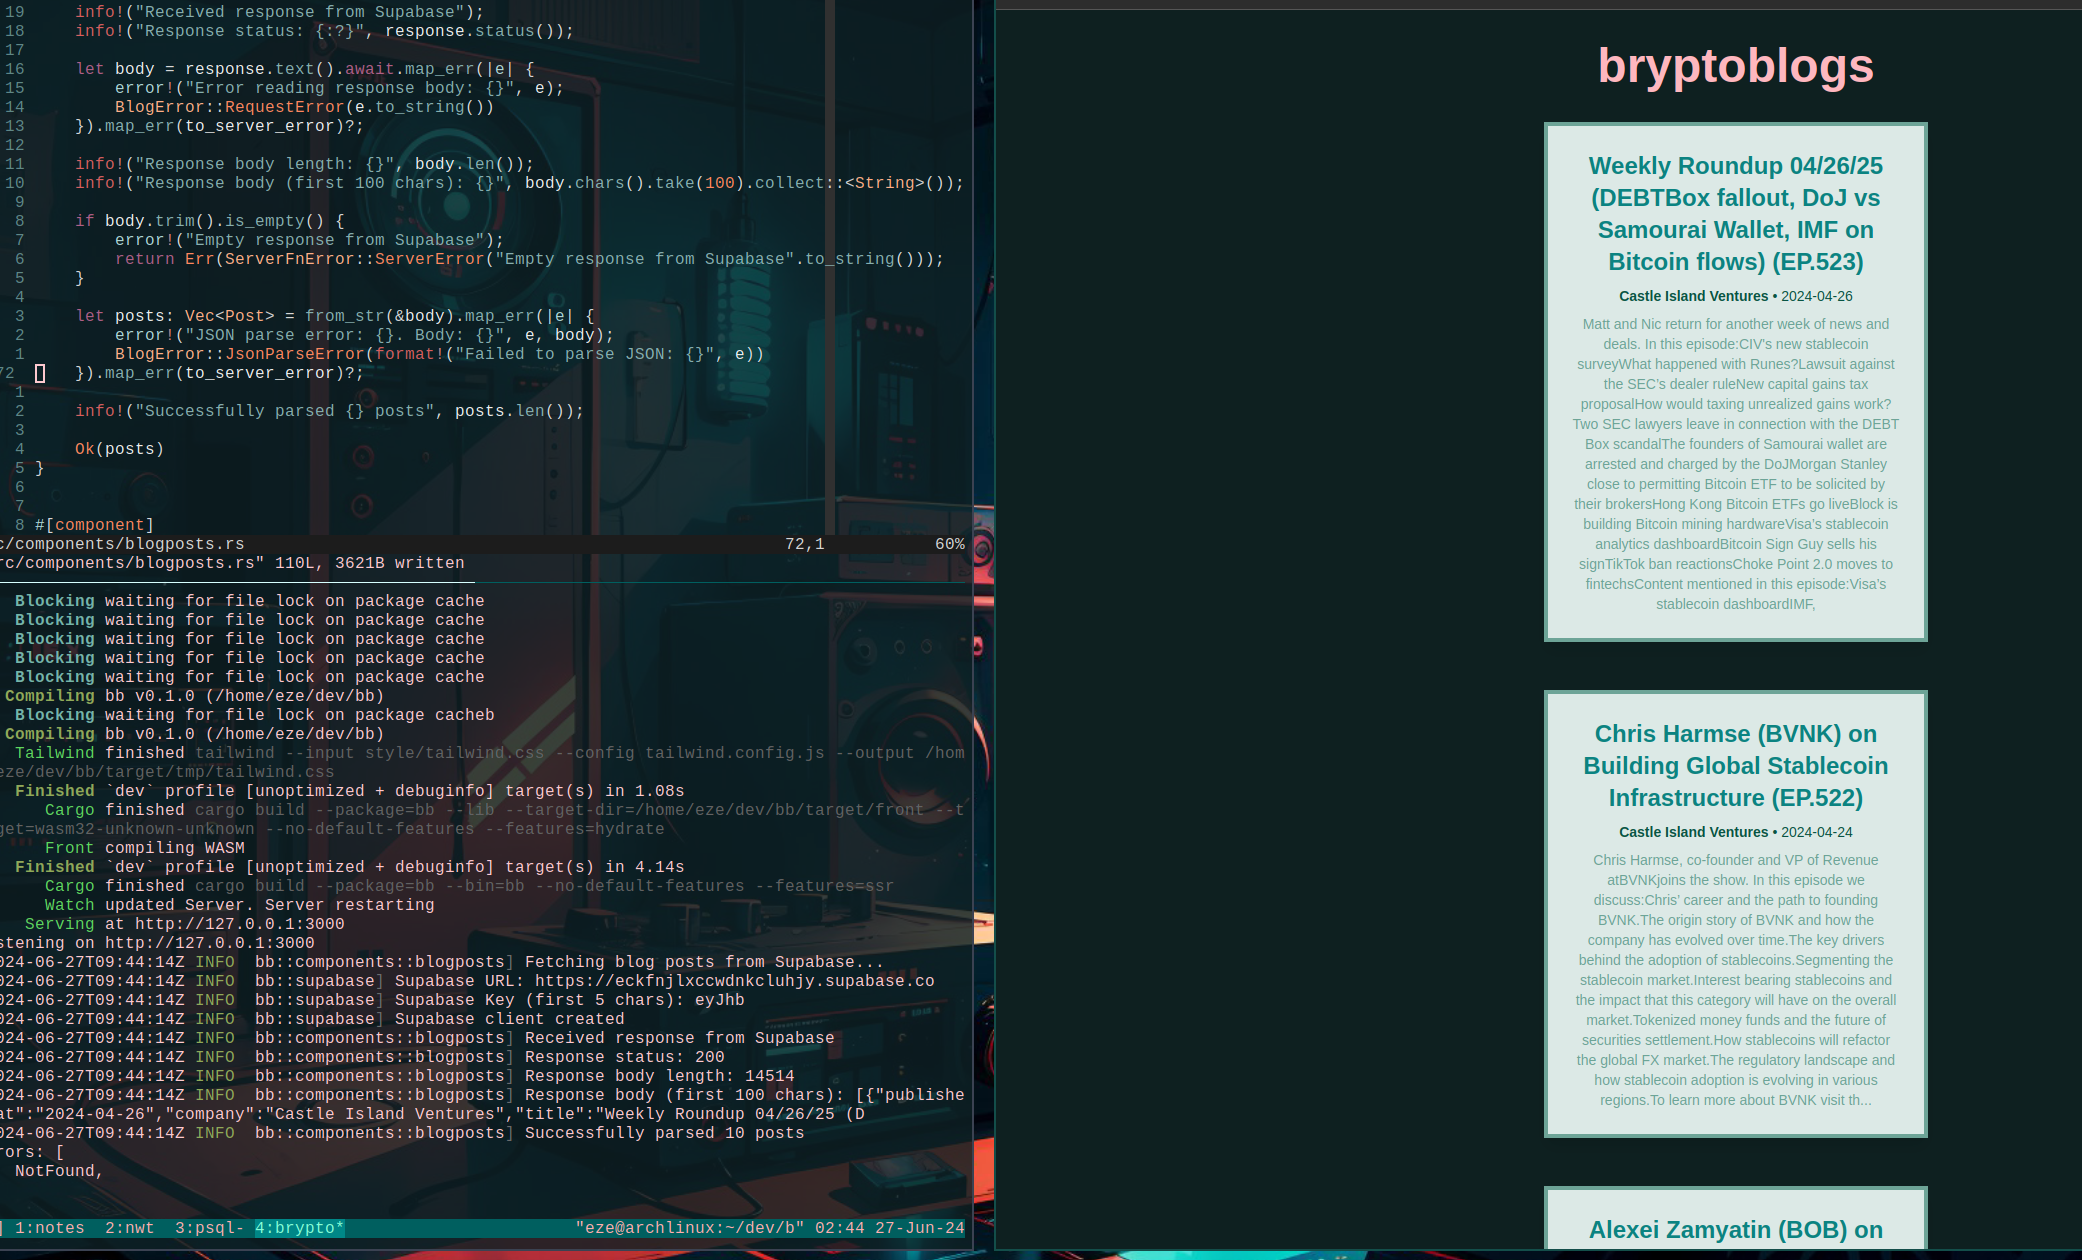
\includegraphics[width=12cm]{bb_we_back}
            \captionsetup{labelfont=bf, textfont=it}
            \caption{we back}
            \label{fig:bb_we_back}
        \end{figure}
    \item i had python woes last i checked on this project so we'll see how this
        goes when trying to update things haha
    \item we are so back (Figure~\ref{fig:bb_we_back_again}
        \begin{figure}[ht]
            \centering
            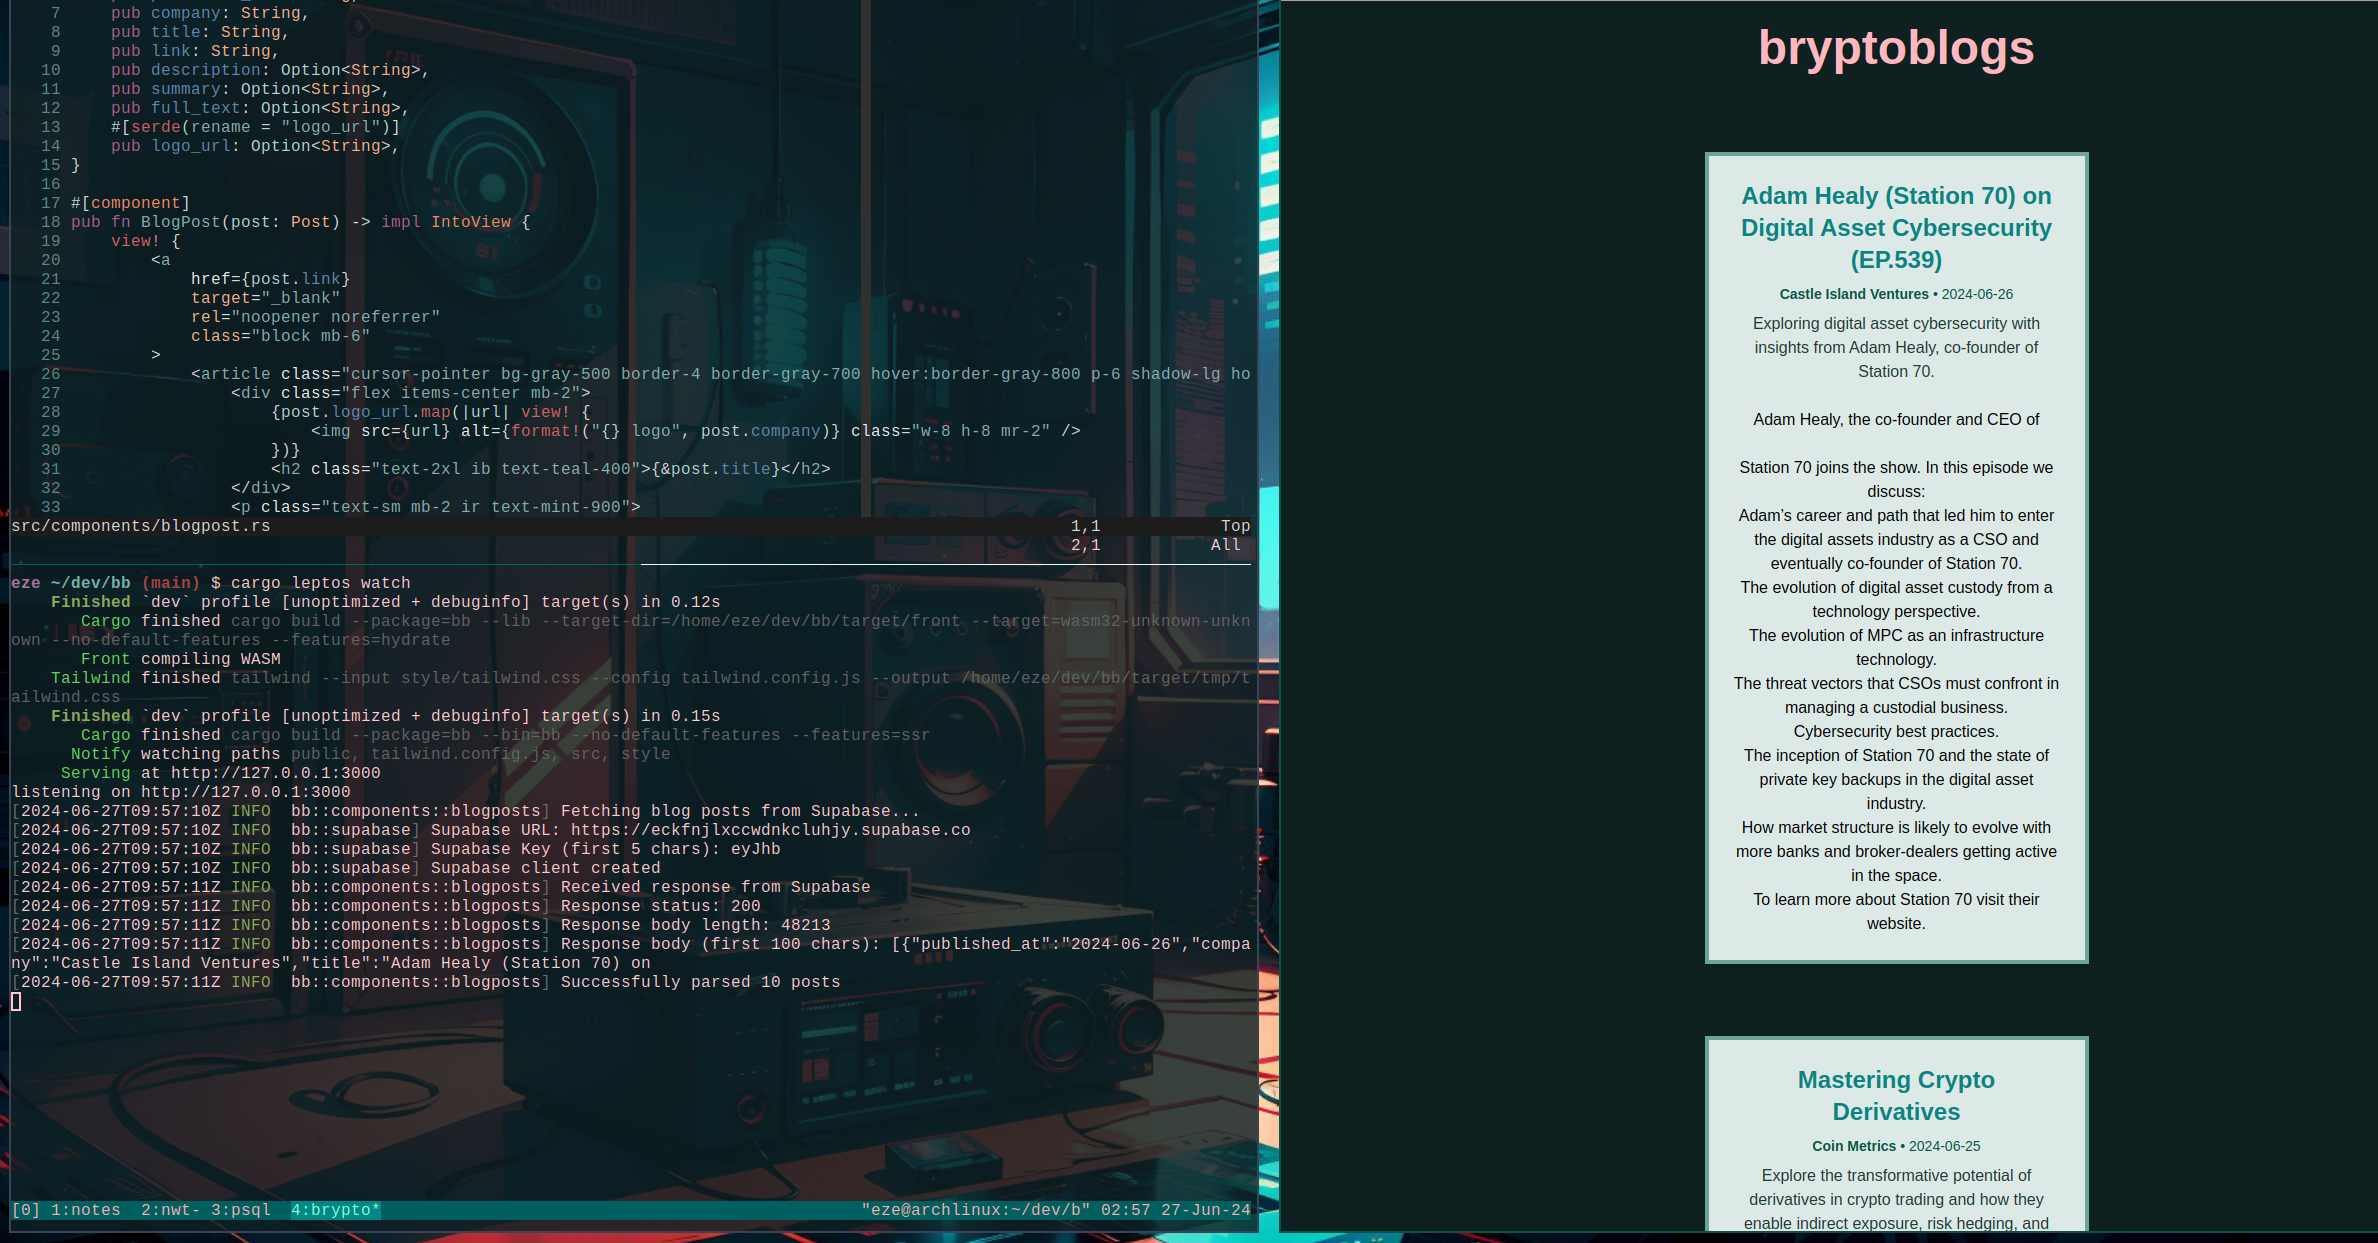
\includegraphics[width=12cm]{bb_we_back_again}
            \captionsetup{labelfont=bf, textfont=it}
            \caption{we so back}
            \label{fig:bb_we_back_again}
        \end{figure}
    \item wow it worked first try, let's goooo. okay this isn't deployed but
        I'll do that next. feels good to revive this project as well in like a
        few hours (i can't search or anything yet, but basic stuff works)

    \clearpage
    \item i am back (in the evening, above was last night technically) working
        on the networktimes leptos rewrite.
    \item added some new models for a new cast list
        \textcolor{blue}{\href{https://github.com/iturner72/thenetworktimes/issues/3}{feature}}.
    \item this feature is just replicating the existing hubble routes used in
        the production site.
    \item i think i will start using github issues to compliment this notes
        document. this stuff is off the dome, and the issue is a more structured
        object. perhaps i can add the relevent pdf pages to the prs once
        features are done, not sure on that yet.
    \item dingllm 

\end{itemize}

\newpage
%%%%%%%%%%%%%%%%%%%%%%%%%%%%%%%%%%%%%%%%%%%%%%%%%%%%%%%%%%%%%%%%%%%%%%%%%%%%%%%
\section{Week 9?}
%%%%%%%%%%%%%%%%%%%%%%%%%%%%%%%%%%%%%%%%%%%%%%%%%%%%%%%%%%%%%%%%%%%%%%%%%%%%%%%
\subsection*{Monday, 07/17/2024}
\begin{itemize}
    \item man i can not count, but we are back. leptos rewrite going well,
        realized i need to use something like
        \texttt{\textcolor{blue}{\href{https://crates.io/crates/deadpool-diesel}{deadpool-diesel}}} since i
        already have some diesel endpoints i want to repurpose and apparently
        this deadpool crate integrates well with tokio (at least better than
        plain r2d2 from diesel)
    \item i will play around with this for article storage and more
    \item looks like deadpool is the move, will explore latest changes to crate
        and try to implement this over \texttt{r2d2}
    \item channels still sus as hell the way i use create_effect, but we will
        send it for now (i don't know how to use \texttt{loom} crate or similar yet to
        test async / concurrent stuff)
\end{itemize}

\newpage
%%%%%%%%%%%%%%%%%%%%%%%%%%%%%%%%%%%%%%%%%%%%%%%%%%%%%%%%%%%%%%%%%%%%%%%%%%%%%%%
\section{Week 8?}
%%%%%%%%%%%%%%%%%%%%%%%%%%%%%%%%%%%%%%%%%%%%%%%%%%%%%%%%%%%%%%%%%%%%%%%%%%%%%%%
\subsection*{Sunday, 06/10/2024}
\begin{itemize}
    \item we might be back (leptos rewrite). notes from testing existing hubble
        node routes with leptos components.
    \item this is not live yet since it has very limited funtionality.
    \item \texttt{fetch_username} checks if \texttt{lead_usernames} already 
        has the \texttt{fid}. if not, it fetches the username and updates the 
        state.
    \item added \texttt{ongoing_requests} to track fetches and avoid multiple 
        requests for the same \texttt{fid}.
    \item Used \texttt{create_effect} to manage side effects, ensuring 
        usernames are fetched only once.
    \item Used \texttt{spawn_local} for async tasks to keep the main thread 
        non-blocking.
    \item \texttt{Signal} and \texttt{set_signal} handle reactive state in the 
        \texttt{Channels} component, making sure the UI updates when data 
        changes.
    \item \texttt{HashSet} tracks \texttt{ongoing_requests}, preventing 
        duplicate fetches and redundant state updates.
    \item The component dynamically displays usernames from the updated state.
    \item asdfasdf
\end{itemize}

\subsection*{Monday, 06/11/2024}
\begin{itemize}
    \item removed the \texttt{lead_username} variable and its assignment using 
        \texttt{unwrap_or_else} from the \texttt{view!} macro.
    \item added closure inside the \texttt{view!} macrothat matches on 
        \texttt{lead_usernames.get().get(&fid)}.
    \item if the lead username is available show it, else show "chill" in div
        where username would be 
    \item closure is defined using \texttt{move ||} to capture the 
        \texttt{lead_usernames} and \texttt{fid} variables.
\end{itemize}

\subsection*{Tuesday, 06/12/2024}
\begin{itemize}
    \item begin rewrite of cast and cast list pages, need to think about using 
        \texttt{create_effect} in the complicated way that i did above.
    \item using this \texttt{create_effect} in the way that i am to sync the
        reactive system is \textit{officially} discouraged since you might shoot
        off your foot with an infinite loop if you don't create something to
        keep track of the ongoing_requests. i liike the chill message though and
        how it could show up at different times for different channels in some
        cases (probably won't be used, but we will see).
    \item i'll do the cast stuff without \texttt{create_effect} to see
        if it's less complicated and achieves virtually the same thing. 
\end{itemize}

\newpage
%%%%%%%%%%%%%%%%%%%%%%%%%%%%%%%%%%%%%%%%%%%%%%%%%%%%%%%%%%%%%%%%%%%%%%%%%%%%%%%
\section{Week 7?}
%%%%%%%%%%%%%%%%%%%%%%%%%%%%%%%%%%%%%%%%%%%%%%%%%%%%%%%%%%%%%%%%%%%%%%%%%%%%%%%
\subsection*{04/20/2024}
\subsection*{Saturday, 04/20/2024}
\begin{itemize}
    \item \textcolor{blue}{\href{https://github.com/queazyg}{Q}} is helping me with ai nyt server.
    \item I am hard stuck on messages so perhaps we will crack it together.
\end{itemize}

\subsection*{Sunday, 04/21/2024}
\begin{itemize}
    \item Got diesel initialized in the project for storing articles, have not
        yet tested the ORM yet, I'll do this soon. 
    \item I was distracted by the reactions feature for the network times. This
        was really easy to add, and I styled it indigo-300 or something like
        this. I've never seen a social site have this color like, so it's
        interesting at least.
    \item You can't yet press the like, this will work once I finally figure out
        how to make the app a valid signer for users.
    \item I added a profile page as shown in Figure~\ref{fig:pfp_page}.
        \begin{figure}[ht]
            \centering
            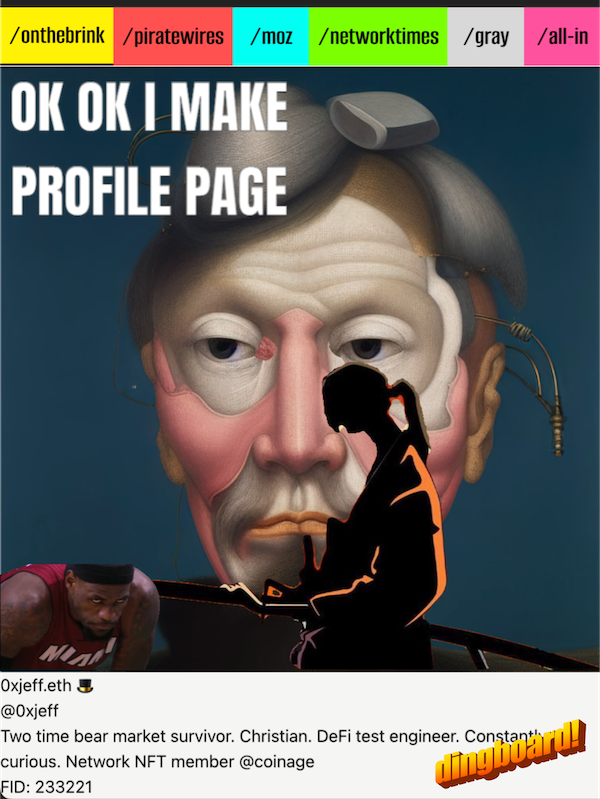
\includegraphics[width=7cm]{pfp_page}
            \captionsetup{labelfont=bf, textfont=it}
            \caption{Profile Page}
            \label{fig:pfp_page}
        \end{figure}
    \item I added hover effects (you can't see it here but matt's pfp background
        has a slight black circle with 10\% opacity applied here
        (Figure~\ref{fig:hover_pfp}).
        \begin{figure}[ht]
            \centering
            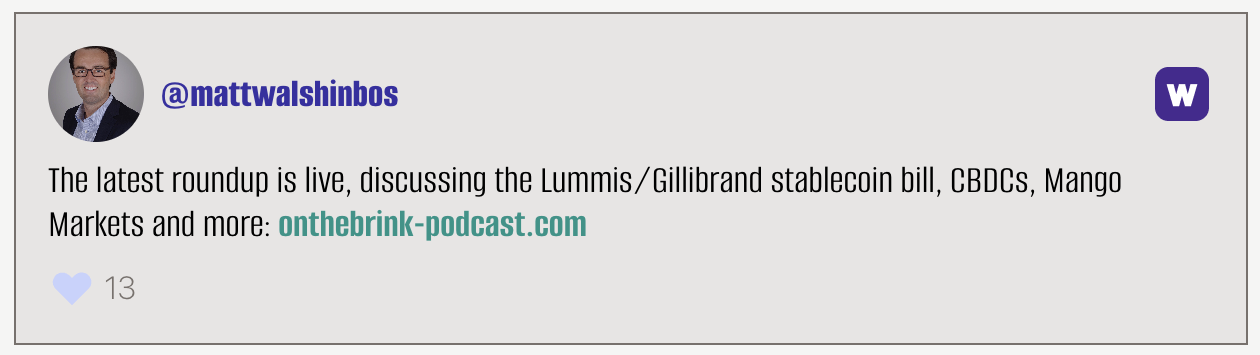
\includegraphics[width=9cm]{hover_pfp}
            \captionsetup{labelfont=bf, textfont=it}
            \caption{Pfp Hover Effect}
            \label{fig:hover_pfp}
        \end{figure}
        \newpage
    \item Distracted once again with iOS app... (Figure~\ref{fig:ios_app_cat})
        \begin{figure}[ht]
            \centering
            
\includegraphics[width=6cm]{ios_app_cat}
            \captionsetup{labelfont=bf, textfont=it}
            \caption{iOS App Cat}
            \label{fig:ios_app_cat}
        \end{figure}
\end{itemize}

\newpage
%%%%%%%%%%%%%%%%%%%%%%%%%%%%%%%%%%%%%%%%%%%%%%%%%%%%%%%%%%%%%%%%%%%%%%%%%%%%%%%
\section{Week 5}
%%%%%%%%%%%%%%%%%%%%%%%%%%%%%%%%%%%%%%%%%%%%%%%%%%%%%%%%%%%%%%%%%%%%%%%%%%%%%%%
\subsection*{I can't be asked}
\begin{itemize}
    \item I am too lazy to summarize my shitty git commits from the 13 til now
        (the 31st).
    \item Enjoy Mr. Incredible Uncanny 4 instead:
    \begin{figure}[ht]
        \centering
        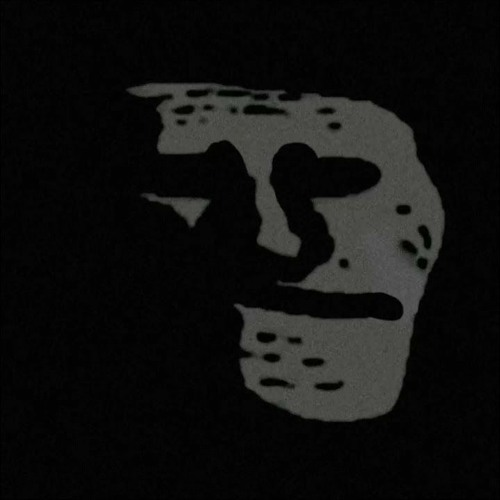
\includegraphics[width=6cm]{uncanny4}
        \captionsetup{labelfont=bf, textfont=it}
        \caption{oooooooooooooooooooo}
        \label{fig:uncanny4}
    \end{figure}
    \item Right, now I've added a few things:
        \begin{itemize}
            \item custom link style and formatting in casts 
            \item render images in casts
            \item sign in with farcaster (doesn't do much else yet)
            \item link to view cast on warpcast 
        \end{itemize}
    \item I suppose I should add reaction data and stuff now.
    \item I'm avoiding the actual hard tech of having the LLM not hallicinate.
        I'm thinking of having a writers room where my proprietary spagetti code
        strips out the things that don't make logical sense from the summary
        from the LLM.
\end{itemize}
\clearpage
\subsection*{I really can't be asked}
\begin{itemize}
    \item I suck at updating this, but I'm focused on a native farcon app at the
        moment. you can check it out
        \textcolor{blue}{\href{https://farcon.info}{here}}.
    \item I'm trying to get messaging working by handcrafting endpoints in rust
        (this will be my downfall, I should just use Neynar) so I'll use them in
        both apps anyways.
    \item Figure~\ref{fig:farcaster_auth} is a drawing (from farcaster YT 
        tutorial) which shows how to create a message with a custom client 
        application.
        \begin{figure}[ht]
            \centering
            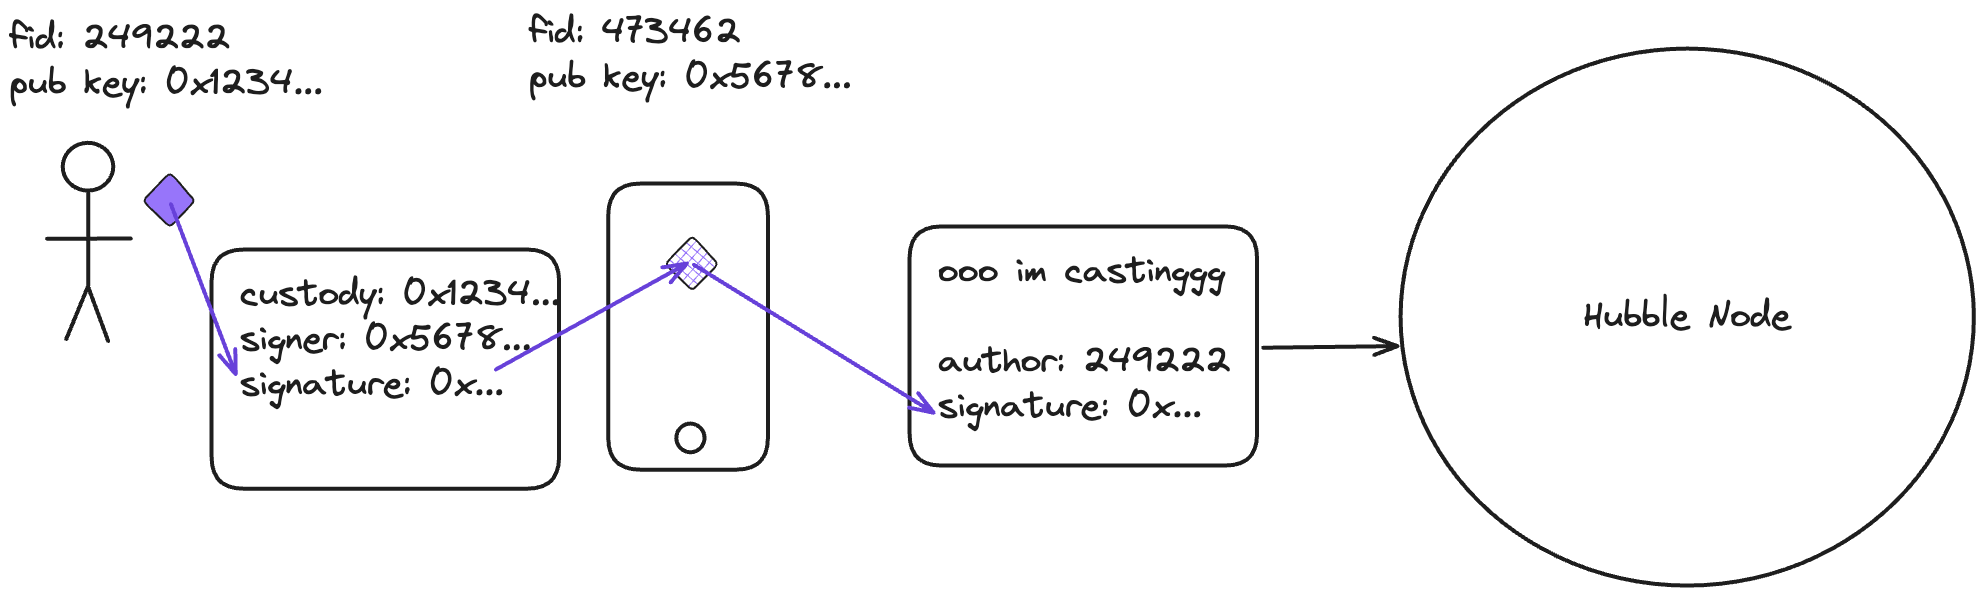
\includegraphics[width=15cm]{farcaster_auth}
            \captionsetup{labelfont=bf, textfont=it}
            \caption{Farcaster Signer Concept}
            \label{fig:farcaster_auth}
        \end{figure}
    \item pinata, farcasterindex, things to thing about using recommended by a
        friend.
\end{itemize}

\newpage
%%%%%%%%%%%%%%%%%%%%%%%%%%%%%%%%%%%%%%%%%%%%%%%%%%%%%%%%%%%%%%%%%%%%%%%%%%%%%%%
\section{Week 4 SEE WEEK 5}
%%%%%%%%%%%%%%%%%%%%%%%%%%%%%%%%%%%%%%%%%%%%%%%%%%%%%%%%%%%%%%%%%%%%%%%%%%%%%%%

\newpage
%%%%%%%%%%%%%%%%%%%%%%%%%%%%%%%%%%%%%%%%%%%%%%%%%%%%%%%%%%%%%%%%%%%%%%%%%%%%%%%
\section{Week 3 - AHHHHH}
%%%%%%%%%%%%%%%%%%%%%%%%%%%%%%%%%%%%%%%%%%%%%%%%%%%%%%%%%%%%%%%%%%%%%%%%%%%%%%%

\subsection*{Monday, 3/11/2024}
\begin{itemize}
    \item See Figure~\ref{fig:uncanny2}.
    \begin{figure}[ht]
        \centering
        
\includegraphics[width=6cm]{uncanny2}
        \captionsetup{labelfont=bf, textfont=it}
        \caption{AHHHH}
        \label{fig:uncanny2}
    \end{figure}
\end{itemize}

\subsection*{Tuesday, 3/12/2024}
\begin{itemize}
    \item See Figure~\ref{fig:uncanny3}.
    \begin{figure}[ht]
        \centering
        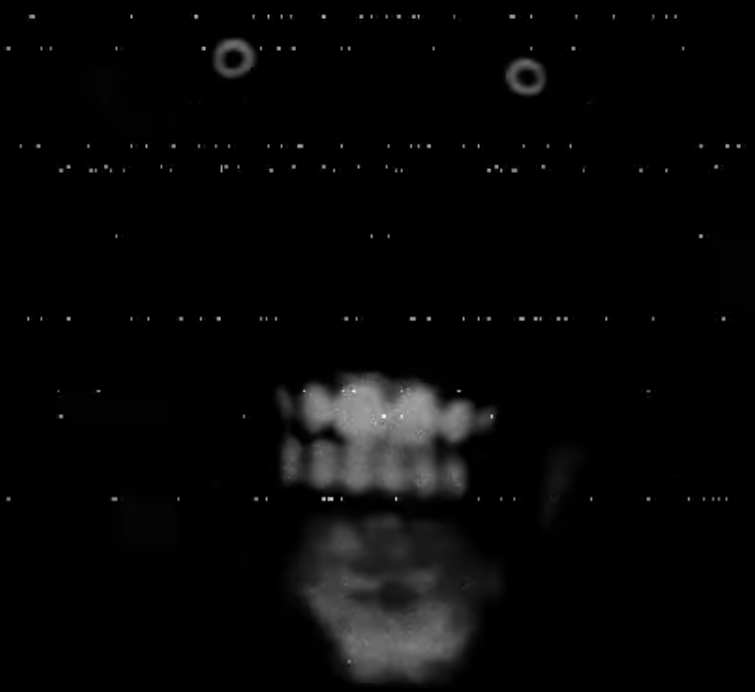
\includegraphics[width=6cm]{uncanny3}
        \captionsetup{labelfont=bf, textfont=it}
        \caption{AHHHHHHHHHHHHHH}
        \label{fig:uncanny3}
    \end{figure}
\end{itemize}

\subsection*{Wednesday, 3/13/2024}
\begin{itemize}
    \item Store articles in local storage to prevent multiple API calls per
        channel per session. Still very clunky behavior with NavBar versus logos
        on ArticleList.
\end{itemize}

\newpage
%%%%%%%%%%%%%%%%%%%%%%%%%%%%%%%%%%%%%%%%%%%%%%%%%%%%%%%%%%%%%%%%%%%%%%%%%%%%%%%
\section{Week 2 - Feature Maxing}
%%%%%%%%%%%%%%%%%%%%%%%%%%%%%%%%%%%%%%%%%%%%%%%%%%%%%%%%%%%%%%%%%%%%%%%%%%%%%%%

\subsection*{Monday, 3/11/2024}
\begin{itemize}
    \item Settle on OVH server to host and migrate away from AWS.
\end{itemize}

\subsection*{Tuesday, 3/12/2024}
\begin{itemize}
    \item Get Claude 3 Opus API working for article gen on photo click.
\end{itemize}

\subsection*{Wednesday, 3/13/2024}
\begin{itemize}
    \item redesign by another 10X designer, Elvia Franco. 
\end{itemize}

\subsection*{Thursday, 3/14/2024}
\begin{itemize}
    \item Skim through \cite{huyen2022designing} for the 4th time.
\end{itemize}

\newpage
%%%%%%%%%%%%%%%%%%%%%%%%%%%%%%%%%%%%%%%%%%%%%%%%%%%%%%%%%%%%%%%%%%%%%%%%%%%%%%%
\section{Week 1 - Ship Website ASAP}
%%%%%%%%%%%%%%%%%%%%%%%%%%%%%%%%%%%%%%%%%%%%%%%%%%%%%%%%%%%%%%%%%%%%%%%%%%%%%%%

\subsection*{Friday, 3/8/2024}
\begin{itemize}
    \item Recruit 10x designer, Michael Raisch.
    \item Set ship or die goal to Sunday (Didn't know the deadline at the time).
    \item Install hubble and run node.
    \item Get basic views built.
    \item Rust server which makes API calls to various LLM models.
\end{itemize}

\subsection*{Saturday, 3/9/2024}
\begin{itemize}
    \item Connect rust server api calls to client components. 
    \item Struggle with hosting server.
\end{itemize}

\subsection*{Sunday, 3/10/2024}
\begin{itemize}
    \item Launch at 6AM rofl.
\end{itemize}


\clearpage
\addcontentsline{toc}{section}{References}
\bibliography{chapters/references} 
\label{sec:references}

\end{document}
